% !TEX root = main.tex

\section{存储器的层次结构}
\subsection{概述}
存储器按照存储方式可分为以下几种:
\begin{enumerate}
	\item 随机访问存储器(RAM)\\
	存储器任意单元可随时访问且访问所需时间相同
	\begin{itemize}
		\item 静态(SRAM):cache\\
		\textbf{触发器};只要加电源,信息就能一直保持;集成度低,引脚多,速度快
		\item 动态(DRAM):主存\\
		\textbf{电容};每隔一段时间必须刷新;现在一般用DDR3 SDRAM(Double Data-Rate Synchronous)
	\end{itemize}
	\item 只读存储器(ROM):BIOS(Basic Input Output System)\\
	正常工作时只读,能随机读出,不能随机写入
	\begin{itemize}
		\item MROM:只读
		\item PROM:一次写
		\item EPROM/EEPROM:多次改写
	\end{itemize}
	\item 相联存储器(Content Addressed Memory, CAM):快表(TLB)\\
	按内容检索到存储位置进行读写
	\item 直接存取存储器(DAS):磁盘\\
	可以直接定位到要读写的数据块,存取时间的长短与数据所在位置有关
	\item 顺序存储器(SAS):磁带\\
	数据按顺序从存储载体的始端读出或写入,存取时间的长短与数据所在位置有关
\end{enumerate}
按照信息的可保存性分为:
\begin{itemize}
	\item 断电后数据是否丢失
	\begin{itemize}
		\item 挥发性(volatile)/易失存储器:SRAM、DRAM
		\item 非挥发性/非易失存储器(NVM):ROM、磁盘、闪存
	\end{itemize}
	\item 读出后是否保存数据
	\begin{itemize}
		\item 破坏性存储器(读出原信息被破坏,需重写):DRAM
		\item 非破坏性存储器:SRAM
	\end{itemize}
\end{itemize}
地址译码两种方式
\begin{enumerate}
	\item 线选法(一位地址译码)\\
	SRAM,只在单方向译码,同时读出一条字线上的所有位,$k$位地址对应$2^k$地址驱动线
	\item 位片式(二维双译码)\\
	$k$位地址对应$2^\frac{k}{2}+2^\frac{k}{2}$条地址驱动线
\end{enumerate}
主存空间的划分
\begin{enumerate}
	\item ROM区:存放系统程序、标准子程序
	\item RAM区:存放用户程序
\end{enumerate}

\subsection{存储容量扩展}
\subsubsection{位扩展}
存储芯片($mk\times n$位/片)构成存储器($mk\times N$位),需要$\lceil N/n\rceil$片\\
字数不变(存储单元个数不变),位数扩展(字长加长)\\
地址线及读写控制线相连接,数据线单独引出,不需外部译码器
\begin{figure}[H]
\centering
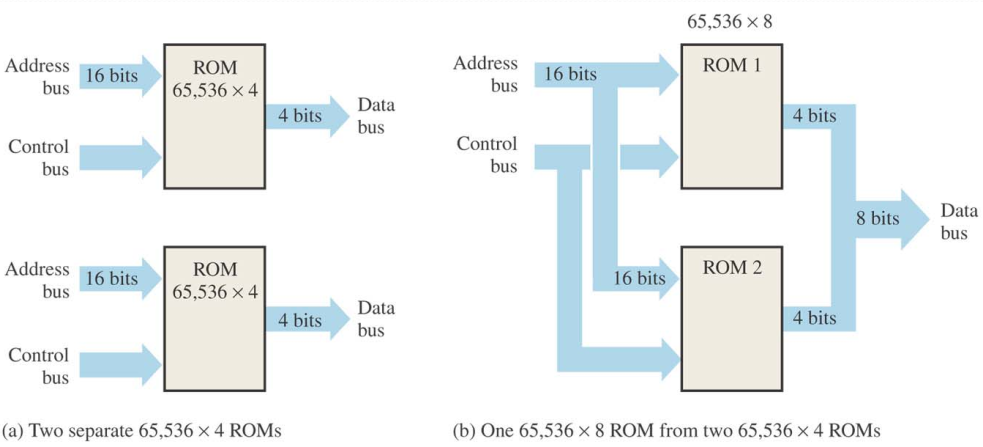
\includegraphics[width=0.6\linewidth]{fig/word-length.PNG}
\end{figure}

\subsubsection{字扩展}
存储芯片($mk\times n$位/片)构成存储器($Mk\times n$位),需要$\lceil M/m\rceil$片\\
位数不变(字长不变),扩充容量(存储单元个数增加)\\
地址线、读写控制线对应相接,片选信号分别与外部译码器各输出端相连
\begin{figure}[H]
\centering
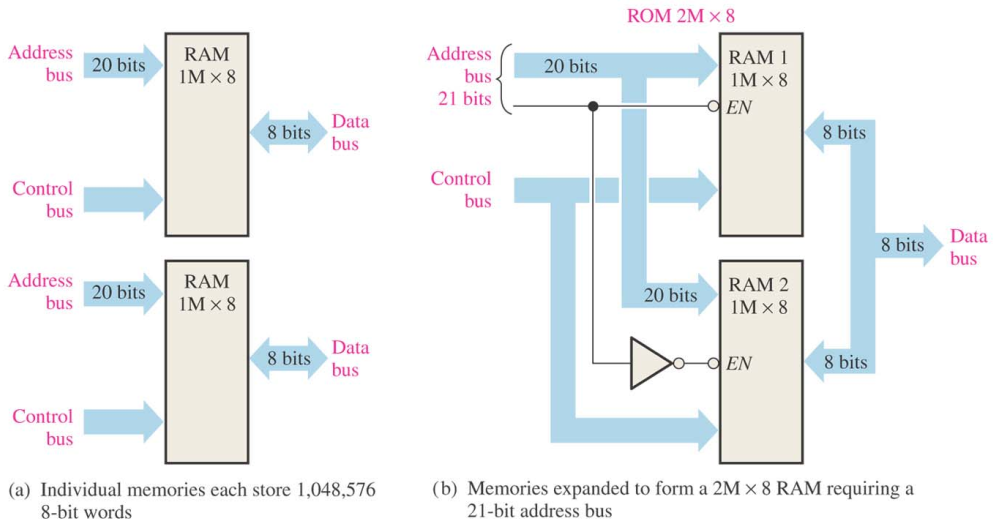
\includegraphics[width=0.6\linewidth]{fig/word-capacity.PNG}
\end{figure}

\subsection{Cache概述}
\subsubsection{计算机存储层次结构}
CPU与cache之间以字为单位传送,cache与主存之间以块为单位传送\\
程序访问局部性
\begin{itemize}
	\item 时间(temporal)局部性
	\item 空间(spatial)局部性
\end{itemize}
cache对程序员是透明的,即程序员在编写程序时无需了解cache是否存在或如何设置

\subsubsection{命中与失效}
\begin{itemize}
	\item 命中(hit):要访问的信息在cache中
	\item 失效(miss):不在cache中
\end{itemize}
平均访问时间
\[\bar{T}=pT_h+(1-p)(T_h+T_m)=T_h+(1-p)T_m\]

\subsection{cache与主存的映射}
cache存放一个主存块的对应单位为行(line)或块(block)或槽(slock)或项(entry)。\\
位宽即为cache一个块的大小,如传送单位为512B,则cache每个块大小为512B
频繁的cache替换称为cache抖动
\subsubsection{直接(direct)映射}
cache内存放的内容是主存的一个子集,因此给出一个主存地址,要在cache中找到这个地址,应该将这个32位地址全部用上。末几位用于确定在cache内存储的位置,高为则用来确定是否为该地址。
注意区别块地址、字地址、字节地址等。
按字索引,后两位不需要。先计算出块地址(因而先模块内数目),再计算块内地址。

\subsubsection{组相联(set associative)映射}
直接模组的数目。
相联度高,缺失率低,但会增加命中时间
只要命中了tag则对应的主存块一定在cache里
\begin{figure}[H]
\centering
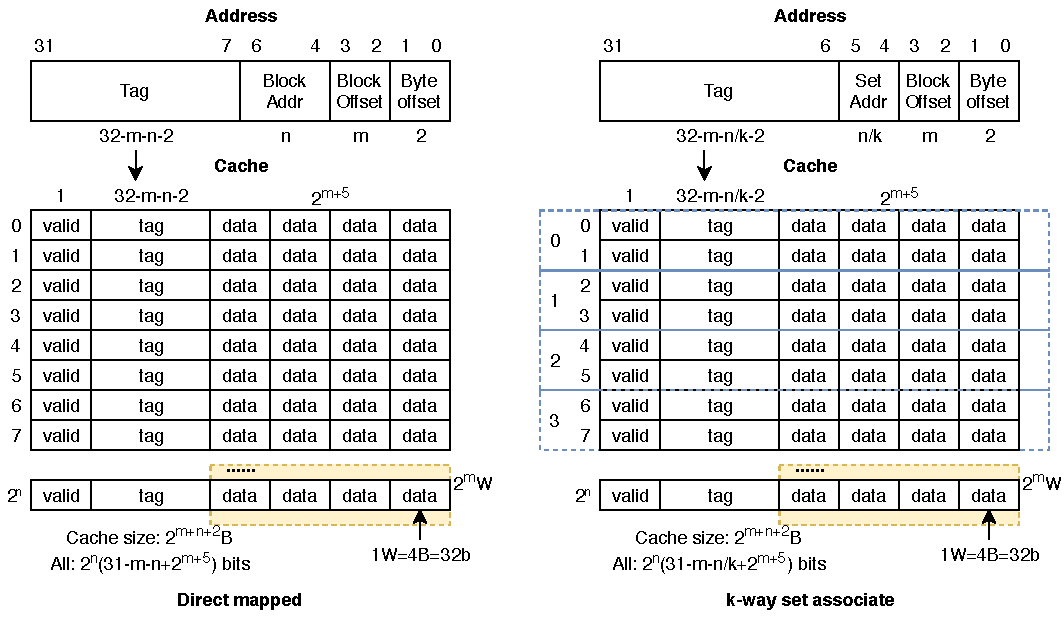
\includegraphics[width=0.8\linewidth]{fig/Cache-combine.pdf}
\end{figure}

\subsection{Cache替换算法}
\begin{itemize}
	\item FIFO
	\item Least Recently Used, LRU
	\item Random
\end{itemize}

\subsection{Cache一致性}
\begin{itemize}
	\item 写命中(hit)
	\begin{itemize}
		\item 写直达(write through):同时写cache和主存\\
		加入写缓冲(write buffer),先存入写缓冲,当写主存操作结束后再将写缓冲数据释放
		\item 写回(write back):只写cache不写主存\\
		每个cache行置一个脏位(dirty bit),若cache行中的主存块被修改,则置为1;只有当脏位为1的块从cache中替换出去时才将其写回主存
	\end{itemize}
	\item 写不命中(miss)
	\begin{itemize}
		\item 写分配(allocate-on-miss):更新主存块相应单元,再将该主存块装入cache(空间局部性)
		\item 写不分配(no-allocate-on-write):直接写主存,不放回
	\end{itemize}
\end{itemize}
通常写直达+写分配/写不分配,写回+写分配

\subsection{多级Cache}
一般L1 Cache为分立Cache(数据指令分开放),减少命中时间获得较短时钟周期\\
L2 Cache为联合Cache,降低缺失率以减少主存缺失损失\\
Intel Core i7采用三级Cache
\begin{center}
\begin{tabular}{|c|c|c|}\hline
L1 & L2 & L3\\\hline
32KB I/ 32 KB D & 256KB & 2MB/core\\\hline
4-way I/8-way D & 8-way & 16-way \\\hline
Pseudo-LRU & Pseudo-LRU & \begin{tabular}{l}Pseudo-LRU\\+ordered selection algorithm\end{tabular}\\\hline
\end{tabular}
\end{center}

\subsection{虚拟存储器}
\subsubsection{概述}
\begin{itemize}
	\item 将内外存统一管理的存储管理机制,按需调页(demand paging)
	\item 虚存是主存和磁盘的抽象,OS使每个进程看到的存储空间都一致
	\item 虚存为每个进程提供一个假象,好像每个进程都独占主存,且主存空间极大
\end{itemize}
\par 分页(paging)基本思想
\begin{itemize}
	\item 将内存分为固定长且较小的存储块,每个进程也划分为固定长度的程序块
	\item 程序块(页/page)可装到存储器可用的存储块(页框/page frame)中
	\item 无需用连续页框来存放一个进程
	\item 操作系统为每个程序/进程生成一个页表(page table)
	\item 通过页表实现逻辑地址到物理地址的转换(address mapping)
\end{itemize}
逻辑地址与物理地址区别
\begin{itemize}
	\item 逻辑地址:程序中指令所用的地址
	\item 物理地址:存放指令或数据实际内存地址
\end{itemize}

\subsubsection{组织方式}
页式虚拟存储器,存在主存中
\begin{itemize}
	\item 指令给出虚拟地址
	\item 每个页表记录对应的虚页情况
	\item valid为0说明缺页(page fault),代价读磁盘,软件处理
	\item CPU执行指令时,先由MMU将逻辑地址转为物理地址
	\item 页大小比cache的block大得多,全相联映射
	\item 写回策略
\end{itemize}
页表结构
\begin{itemize}
	\item 每个进程一个页表
	\item 页表项数由进程大小决定
	\item 页表在主存的首地址记录在页表
\end{itemize}

\subsubsection{快表(TLB)}
转换后备缓冲器(Translation-Lookaside Buffer),存在cache中\\
每次读写操作都至少带来两次存储器访问,一次访问页表,一次访问所需的数据或指令\\
使用cache来存储页表项,它包含了最近使用的那些页表项\\
不可能页表miss了,快表hit了,因为页表缺失,信息一定不在主存页不在cache
\begin{figure}[H]
\centering
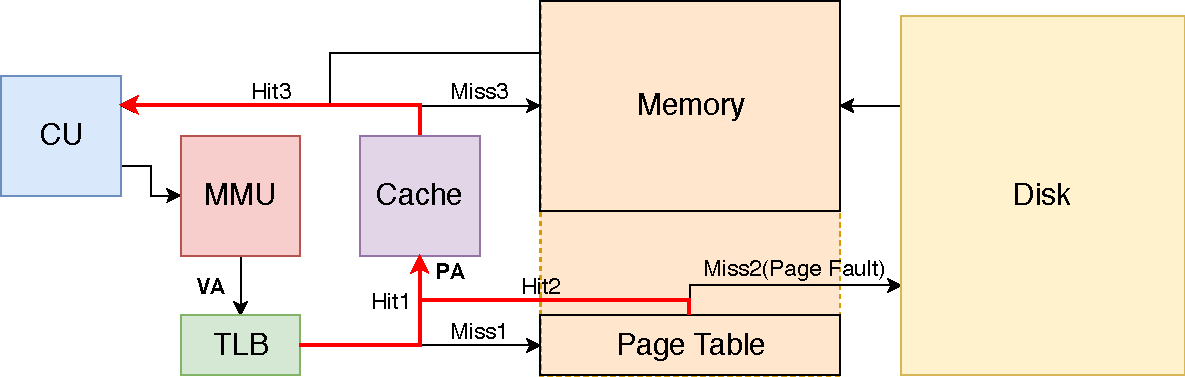
\includegraphics[width=0.8\linewidth]{fig/Cache-page.pdf}
\end{figure}
TLB全相联,有有效位、脏位
\begin{figure}[H]
\centering
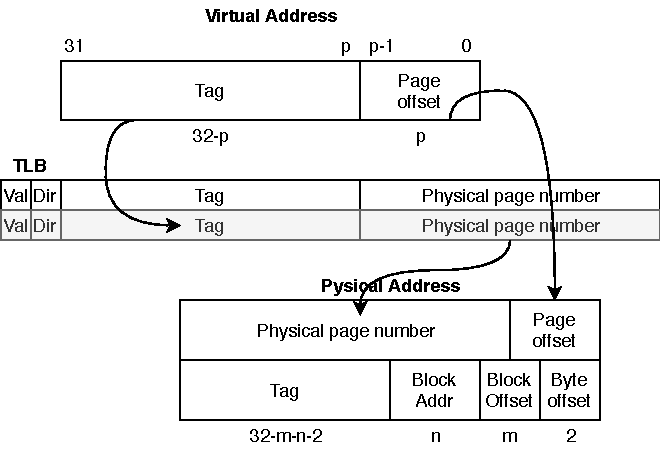
\includegraphics[width=0.6\linewidth]{fig/Cache-page_address.pdf}
\end{figure}